This section investigates the effect of distance on throughput, delay and loss
within a single user, single access point system.

\par The throughput, shown below, is constant for the user from distances
between 0 and 110 meters from the access point. Packet loss occurs at
approximately 120 meters, giving greatly decreased throughput. Between 130 and
150 meters, there are no packets received, giving a throughput of 0Kbps.

\begin{gather*}
	Throughput=\frac{rxPackets*1000*8}{txTime} \\
	TP_{0-110}=\frac{400*1000*8}{20}\\
	= 160Kbps\\
	TP_{120}= \frac{13*1000*8}{20}\\
	= 5.2Kbps \\
	TP_{130-150}=\frac{0*1000*8}{20}\\
	= 0Kbps
\end{gather*}
\captionof{equation}{Average Throughput (Kbps) over distances of 0-150m}

The drop of in the throughput is clearly visible within the plot of Figure
\ref{fig:QBthroughput}.

\begin{figure}[H]
	\centering
	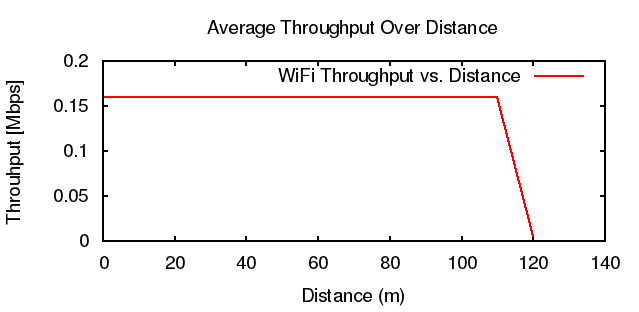
\includegraphics[width=0.8\textwidth]{images/EE500/QB/Images/wifi-throughput}
	\caption{Throughput as measured at distances between 0 and 150 meters}
	\label{fig:QBthroughput}
\end{figure}

The delay, whose values are shown below as read from the database file, begins
to increase at a faster rate between 80 and 110 meters, with much greater
increases between 110 and 120 meters.
\begin{gather*}
	\overline{delay}_0=271582ns \\
	\overline{delay}_{10}=271615ns \\
	\overline{delay}_{20}=271648ns \\
	\overline{delay}_{30}=397353ns \\
	\overline{delay}_{40}=381876ns \\
	\overline{delay}_{50}=490381ns \\
	\overline{delay}_{60}=605123ns \\
	\overline{delay}_{70}=649954ns \\
	\overline{delay}_{80}=835599ns \\
	\overline{delay}_{90}=1279691ns \\
	\overline{delay}_{100}=1574269ns \\
	\overline{delay}_{110}=1723305ns \\
	\overline{delay}_{120}=9362323ns \\
\end{gather*}
\captionof{equation}{Average Delay (ns) over distances of 0-150m}

Beyond a distance of 120m, due to there being a throughput of 0Kbps, there is no
delay value. These values can be seen in Figure \ref{fig:QBdelay}

\begin{figure}[H]
	\centering
	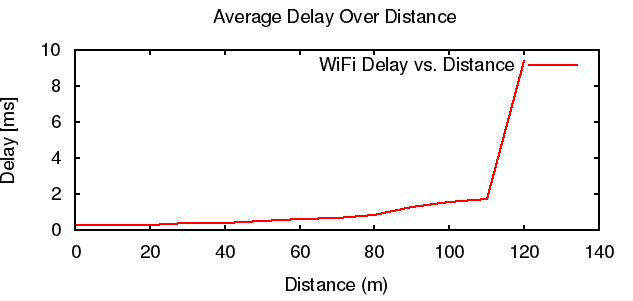
\includegraphics[width=0.8\textwidth]{images/EE500/QB/Images/wifi-delay}
	\caption{Delay as measured at distances between 0 and 150 meters}
	\label{fig:QBdelay}
\end{figure}

For distances between 0 and 110 meters, there is no packet loss due to, as discussed
earlier, all of the packets transmit by the access point are received by the
user.

\par For a distance of 120 meters, the user experiences loss of 96.75\%, and for
distances greater than this, experiences loss of 100\%.

\par The calculations for the packet loss ratio can be seen below:

\begin{gather*}
	PLR=\frac{lostPackets}{rxPackets+lostPackets} \\
	TP_{0-110}=\frac{0}{400+0}\\
	= 0 \\
	TP_{120}= \frac{387}{13+387}\\
	= 0.9675 \\
	TP_{130-150}=\frac{400}{0+400}\\
	= 1
\end{gather*}
\captionof{equation}{Packet Loss Ratio over distances of 0-150m}

\begin{figure}[H]
	\centering
	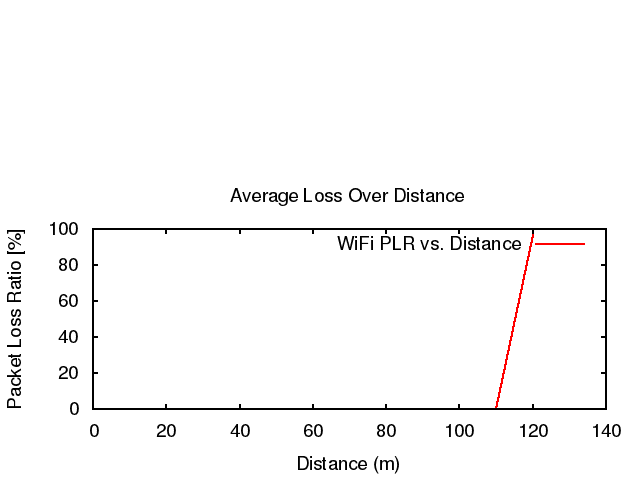
\includegraphics[width=0.8\textwidth]{images/EE500/QB/Images/wifi-loss}
	\caption{Packet Loss Ratio as measured at distances between 0 and 150
	meters}
	\label{fig:QBloss}
\end{figure}
